\documentclass[aspectratio=169]{beamer}

% Je kan het lettertype iets vergroten door hierboven optie ``14pt'' toe te
% voegen.

%==============================================================================
% Aanloop
%==============================================================================

%---------- Vormgeving --------------------------------------------------------

\usetheme{hogent}

% Kies hieronder een achtergrondkleur
\usecolortheme{hgwhite} % witte achtergrond, zwarte tekst
%\usecolortheme{hgblack} % zwarte achtergrond, witte tekst

%---------- Packages ----------------------------------------------------------

\usepackage[dutch]{babel}      % Nederlandse taal: splitsingen, enz.

\usepackage{booktabs}          % Mooie tabellen
\usepackage{multirow,multicol} % Tabelcellen samenvoegen
\usepackage{eurosym}           % Euro symbool

%---------- Commando-definities -----------------------------------------------

%---------- Info over de presentatie ------------------------------------------

\title[Korte titel]{Microservice integration patterns op SAP order-to-cash proces.}
\subtitle{Welke invloed hebben microservices op een order-to-cash proces?}
\author{Lyva Van Damme (\href{mailto:lyva.vandamme.y7102@student.hogent.be}{lyva.vandamme.y7102@student.hogent.be})}
\date{\today}

%==============================================================================
% Inhoud presentatie
%==============================================================================

\begin{document}

%---------- Titelpagina, inhoudstafel -----------------------------------------

\frame{\maketitle}

\begin{frame}
  \frametitle{Inhoud.}

  \tableofcontents
\end{frame}
 
%---------- INLEIDING ------------------------------------------------------------

\section{Inleiding}

\begin{frame}
  \frametitle{Waarom microservices en het order-to-cash proces?}
  
  \begin{itemize}
	  \item Opkomende technologie
	  \item Een gekend proces
	\end{itemize}
\end{frame}

%---------- STAND VAN ZAKEN ------------------------------------------------------------

\section{Stand van zaken}

%--------- microservices
\begin{frame}
	\frametitle{Microservices}
	\begin{itemize}
		\item Definitie
		\item Belang van microservices
		\item Algemene aanpak om microservices te implementeren
		\item Voordelen en nadelen
	\end{itemize}

\end{frame}

\begin{frame}
	\frametitle{Microservices: Definitie}
	\begin{itemize}
		\item Monolithic
		\item Microservice
	\end{itemize}

\end{frame}

\begin{frame}
	\begin{figure}
		\caption{Een monolithic vergeleken met een microservice.}
		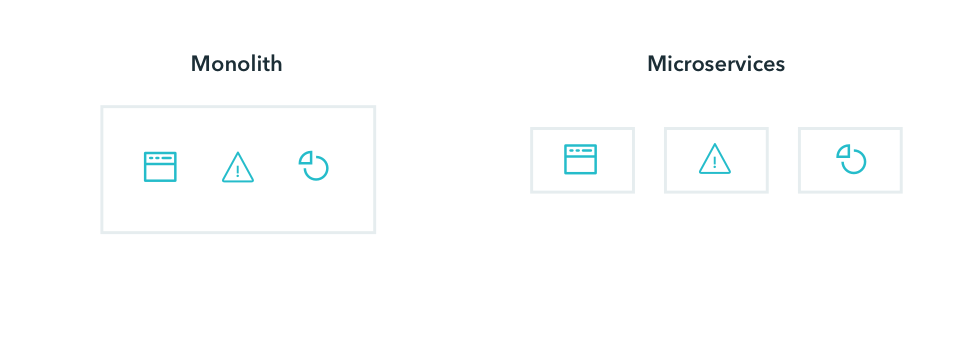
\includegraphics[height=.8\textheight]{img/Mono_Micro.png}
		% Bron afbeelding: https://www.pexels.com/photo/hand-on-cup-of-coffee-984536/
		\label{img:monolithic_microservices}
	\end{figure}
\end{frame}


\begin{frame}
	\frametitle{Belang van microservices}
	\begin{itemize}
		\item De verschillende manier van bescherming
		\item Authenticatie en authorisatie
	\end{itemize}
\end{frame}

\begin{frame}
	\begin{figure}
		\caption{Authenticatie en authorisatie.}
		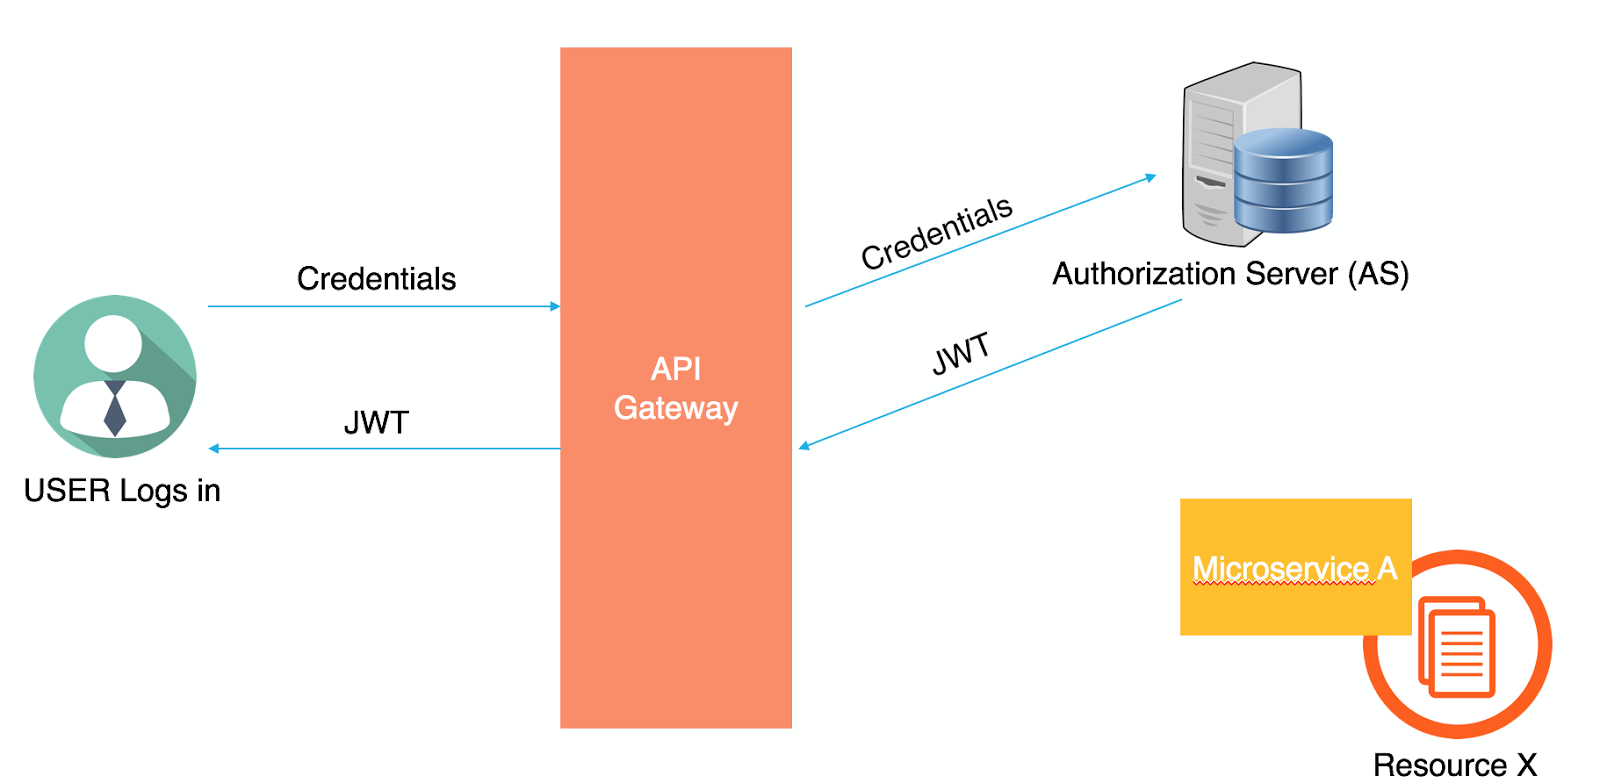
\includegraphics[height=.8\textheight]{img/apiGateway_facadePattern.png}
		% Bron afbeelding: https://www.pexels.com/photo/hand-on-cup-of-coffee-984536/
		\label{img:APIgateway}
	\end{figure}
\end{frame}

\begin{frame}
	\frametitle{Belang van microservices}
	\begin{itemize}
		\item De verschillende manier van bescherming
		\item Authenticatie en authorisatie
		\item Verband met Agile en DevOps
		\item Monitoren van microservices
	\end{itemize}
\end{frame}

\begin{frame}
	\frametitle{Algemene aanpak om microservices te implementeren}
	Voor het overschakelen:
	\begin{itemize}
		\item Hoe zijn andere bedrijven overgeschakeld?
		\item Ervaring van anderen nagaan
		\item Plan opmaken
	\end{itemize}

\end{frame}

\begin{frame}
	\begin{figure}
		\caption{1. Serve a business purpose.}
		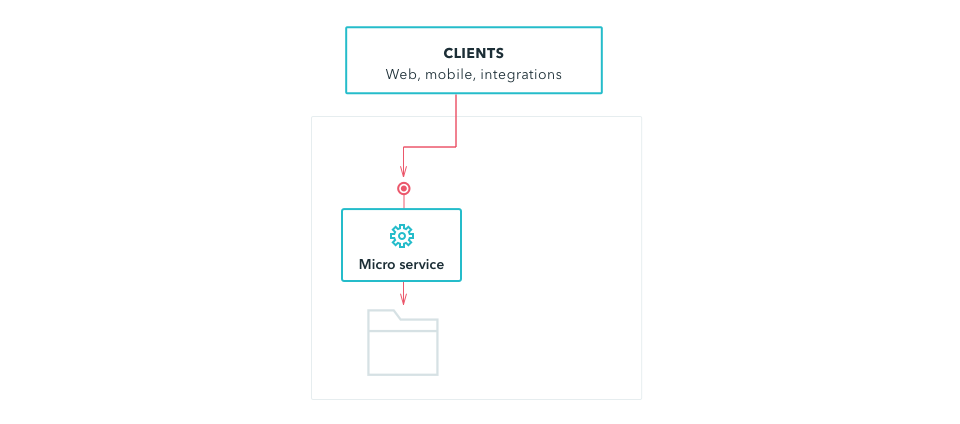
\includegraphics[height=.8\textheight]{img/1.png}
		% Bron afbeelding: https://www.pexels.com/photo/hand-on-cup-of-coffee-984536/
		\label{img:serveABusinessPurpose}
	\end{figure}
\end{frame}

\begin{frame}
	\begin{figure}
		\caption{2. Protect your stuff.}
		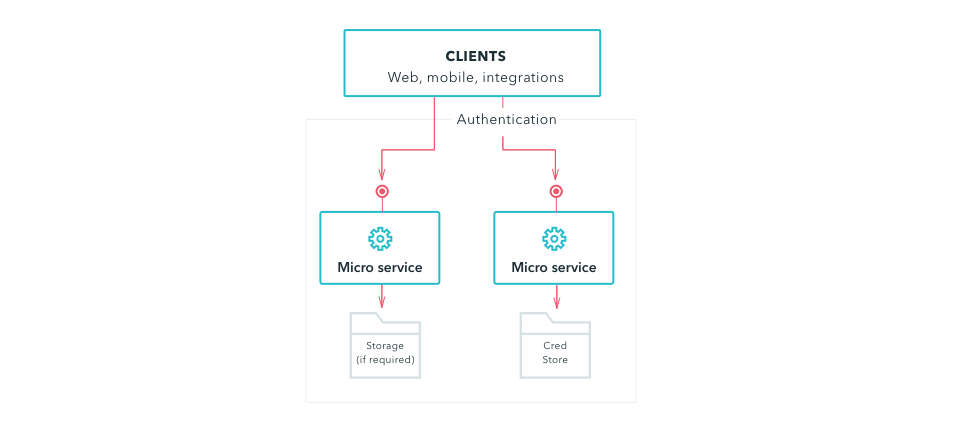
\includegraphics[height=.8\textheight]{img/2.png}
		% Bron afbeelding: https://www.pexels.com/photo/hand-on-cup-of-coffee-984536/
		\label{img:protectYourStuff}
	\end{figure}
\end{frame}

\begin{frame}
	\begin{figure}
		\caption{3. See no evil, hear no evil.}
		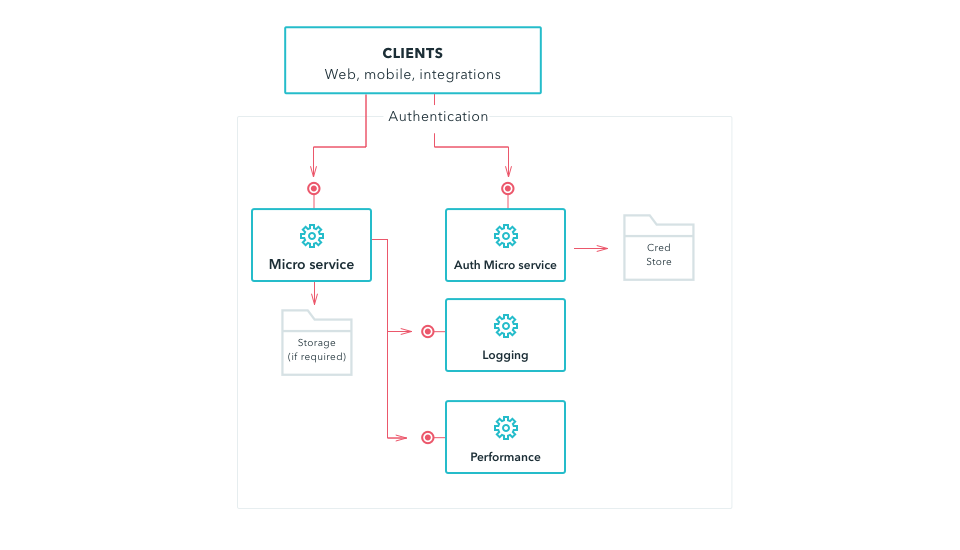
\includegraphics[height=.8\textheight]{img/3.png}
		% Bron afbeelding: https://www.pexels.com/photo/hand-on-cup-of-coffee-984536/
		\label{img:seeNoEvilHearNoEvil}
	\end{figure}
\end{frame}

\begin{frame}
	\begin{figure}
		\caption{4. Find your stuff}
		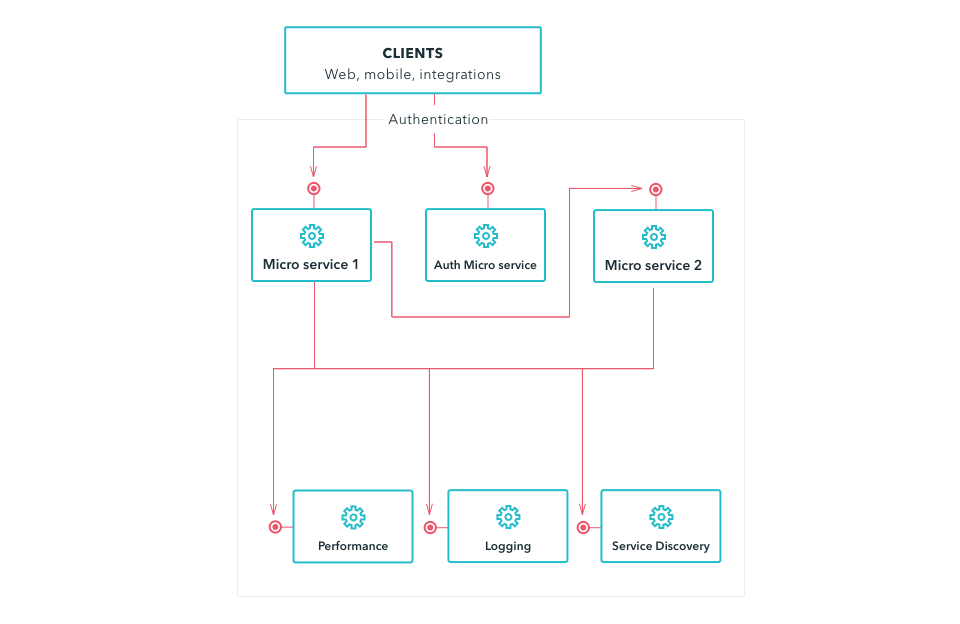
\includegraphics[height=.8\textheight]{img/4.png}
		% Bron afbeelding: https://www.pexels.com/photo/hand-on-cup-of-coffee-984536/
		\label{img:findYourStuff}
	\end{figure}
\end{frame}

\begin{frame}
	\begin{figure}
		\caption{5. Create a gateway}
		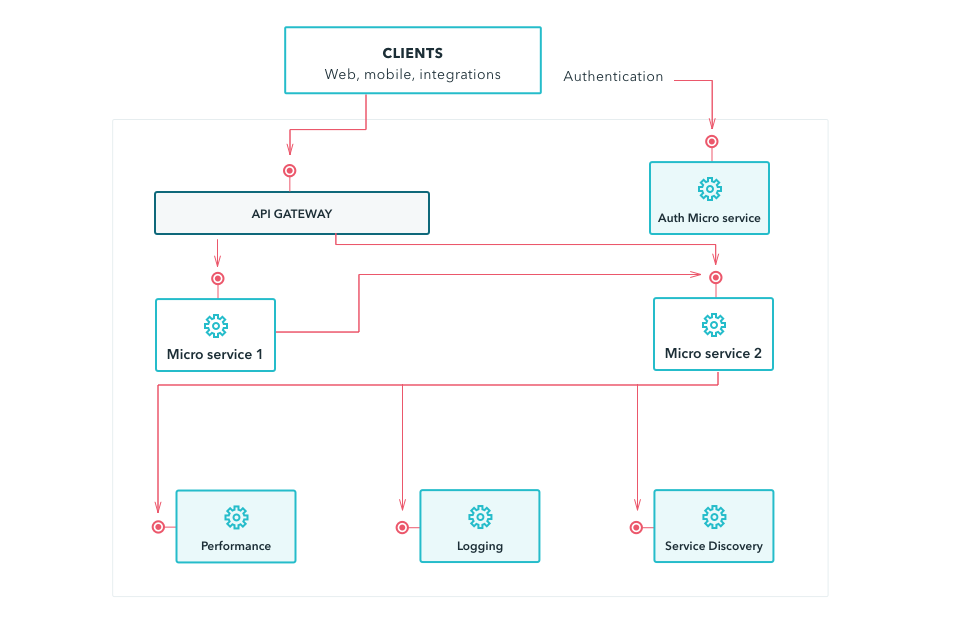
\includegraphics[height=.8\textheight]{img/5.png}
		% Bron afbeelding: https://www.pexels.com/photo/hand-on-cup-of-coffee-984536/
		\label{img:createAGateway}
	\end{figure}
\end{frame}

\begin{frame}
	\begin{figure}
		\caption{6. Construct events}
		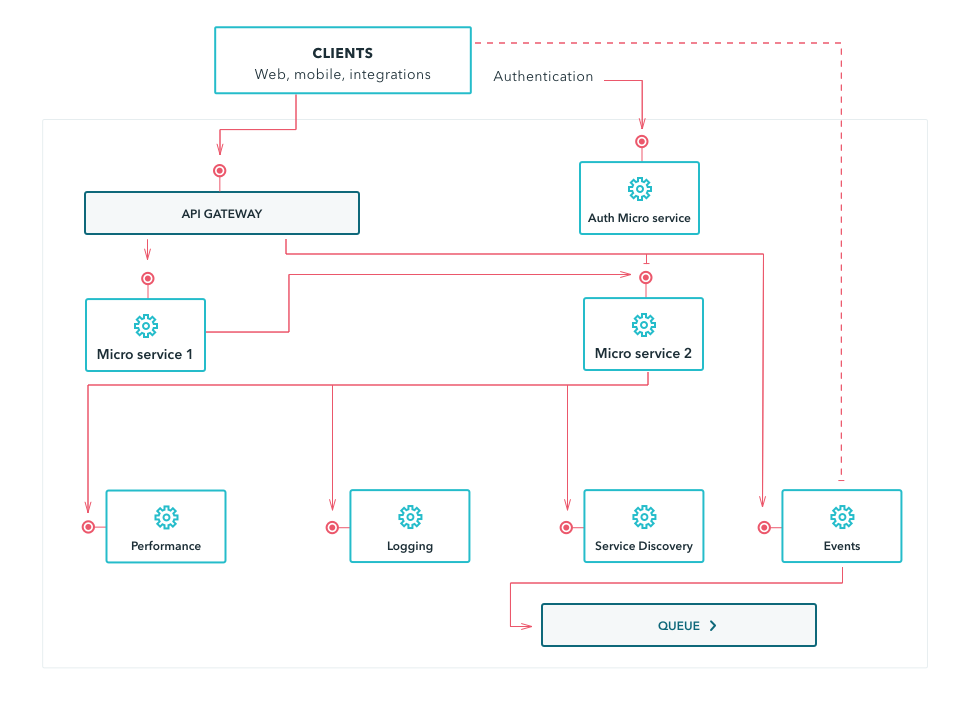
\includegraphics[height=.8\textheight]{img/6.png}
		% Bron afbeelding: https://www.pexels.com/photo/hand-on-cup-of-coffee-984536/
		\label{img:constructEvents}
	\end{figure}
\end{frame}

\begin{frame}
	Aandachtspunten bij overschakeling:
	\begin{itemize}
		\item Is de overschakeling noodzakelijk?
		\item Zijn er teamleden die er al mee gewerkt hebben?
		\item Staat iedereen achter de verandering?
		\item Onderschat het niet!
	\end{itemize}
\end{frame}

\begin{frame}
	\frametitle{Voordelen en nadelen}
	\begin{table}
		\begin{tabular}{p{6cm} p{6cm}}
			\textbf{Voordelen} & \textbf{Nadelen} \\
			\midrule
			Architectuur wordt flexibeler & Het concept bij nieuwe technologie is niet altijd duidelijk              \\
			\midrule
			Hermodelleren van de architectuur is eenvoudiger    & Brengt complexiteit met zich mee   \\
			\midrule
			Geen onnodige stappen maken & Debuggen en fouten vinden is moeilijk              \\
			\midrule
			Microservices zijn onafhankelijk    &    \\
			\midrule
			Snelheid van de architectuur verbeterd &               \\
			\bottomrule
		\end{tabular}
		
		\label{tab:voorbeeld}
		\caption{De voordelen en nadelen van microservices}
	\end{table}

\end{frame}

%--------- Order-to-cash proces
\begin{frame}
	\frametitle{Order-to-cash proces}
	\begin{itemize}
		\item Definitie
		\item Technologie
	\end{itemize}

\end{frame}

\begin{frame}
	\frametitle{Order-to-cash: Definitie}
	\begin{figure}
		\caption{Order-to-cash proces}
		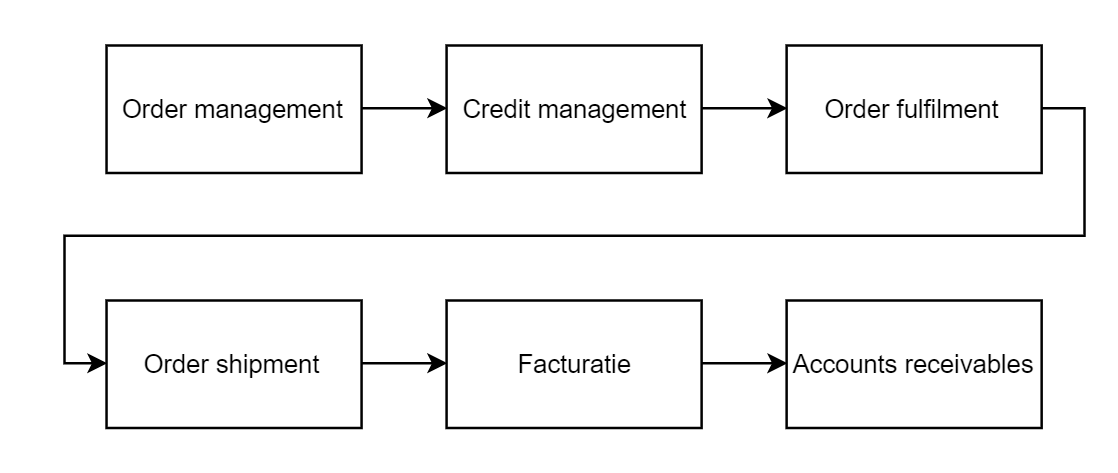
\includegraphics[height=.8\textheight]{img/OTC.png}
		% Bron afbeelding: https://www.pexels.com/photo/hand-on-cup-of-coffee-984536/
		\label{img:Order-to-cash proces}
	\end{figure}
\end{frame}

\begin{frame}
	\frametitle{Order-to-cash: Technologie}
	SAP biedt Kyma aan.
	\begin{itemize}
		\item Open-source project.
		\item Cloud-based en on-premise applicaties.
		\item Betere end-to-end ervarings scenario's.
		\item Kleine modules developpen.
	\end{itemize}
\end{frame}

\begin{frame}
	Eigenschappen van Kyma
	\begin{itemize}
		\item Be open and extendable
		\item Be seamlessly connected
		\item Use any programming language
		\item Bring speed and agility
		\item Accelerate innovation
	\end{itemize}
\end{frame}

\begin{frame}
	\frametitle{Requirements van de business}
	\begin{itemize}
		\item Orders plaatsen
		\item Order ophalen uit voorraad
		\item Goed voorraadbeheer
		\item Levering moet goed gepland worden
		\item Facturatie moet goed beheerd worden
		\item De betaling moeten in het oog gehouden worden
	\end{itemize}
\end{frame}
%---------- METHODOLOGIE ------------------------------------------------------------

\section{Methodologie}

\begin{frame}
	\frametitle{Methodologie}
	\begin{itemize}
		\item Termen toelichten
		\item Microservices binnen het order-to-cash proces
		\item Databank structuur
		\item De complete architectuur opbouwen
	\end{itemize}

\end{frame}

\begin{frame}
	\frametitle{Termen}
	\begin{itemize}
		\item Queue
		\item Overhead
		\item Datastore
	\end{itemize}

\end{frame}

\begin{frame}
	\frametitle{Microservices binnen het order-to-cash proces}
	\begin{itemize}
		\item De microservices van het order-to-cash proces met hun onderliggende communicatie.
		\item Communciatie methode tussen microservices
	\end{itemize}
\end{frame}

\begin{frame}
	\frametitle{De microservices van het order-to-cash proces.}
	\begin{itemize}
		\item Klanten gegevens ophalen
		\item Orders plaatsen, ophalen en verwijderen
		\item Producten ophalen en het aantal in voorraad veranderen
		\item Facturatie maken en ophalen
		\item Shipment documentatie opstellen
		\item Aanmaning opmaken en verwijderen
		\item Berichten plaatsen op de queue
		\item Berichten ophalen van de queue
	\end{itemize}
\end{frame}

\begin{frame}
	\frametitle{De communciatie methode tussen microservices}
	\begin{figure}
		\caption{Voorbeeld van de communicatie}
		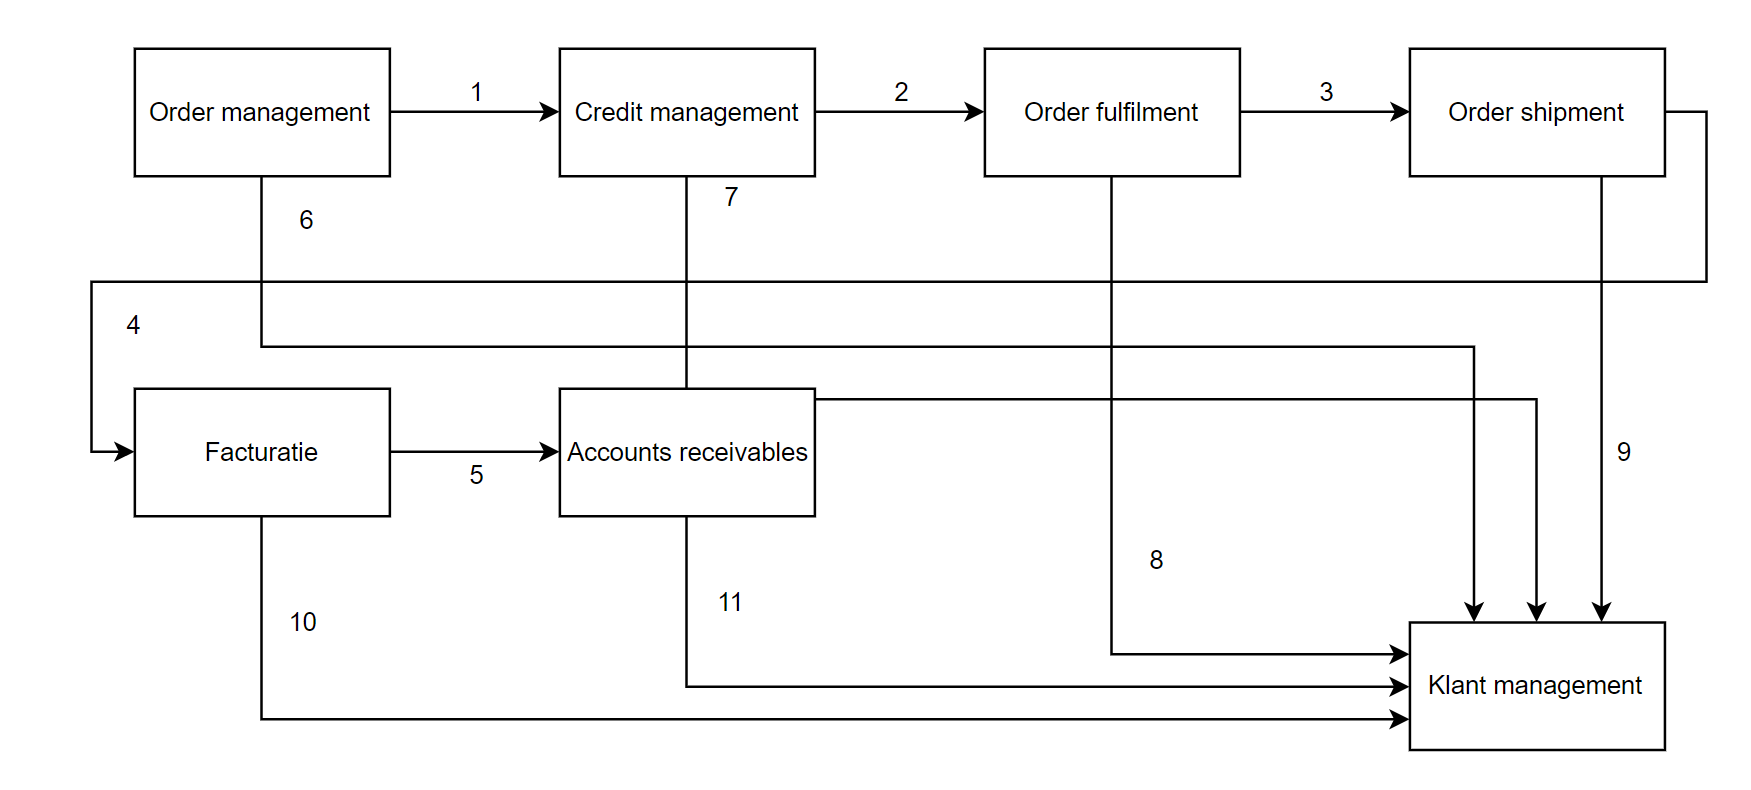
\includegraphics[height=.8\textheight]{img/schema_communicatie.png}
		% Bron afbeelding: https://www.pexels.com/photo/hand-on-cup-of-coffee-984536/
		\label{img:voorbeeldCommunicatie}
	\end{figure}
\end{frame}

\begin{frame}
	\frametitle{Databank structuur}
	\begin{figure}
		\caption{Databank}
		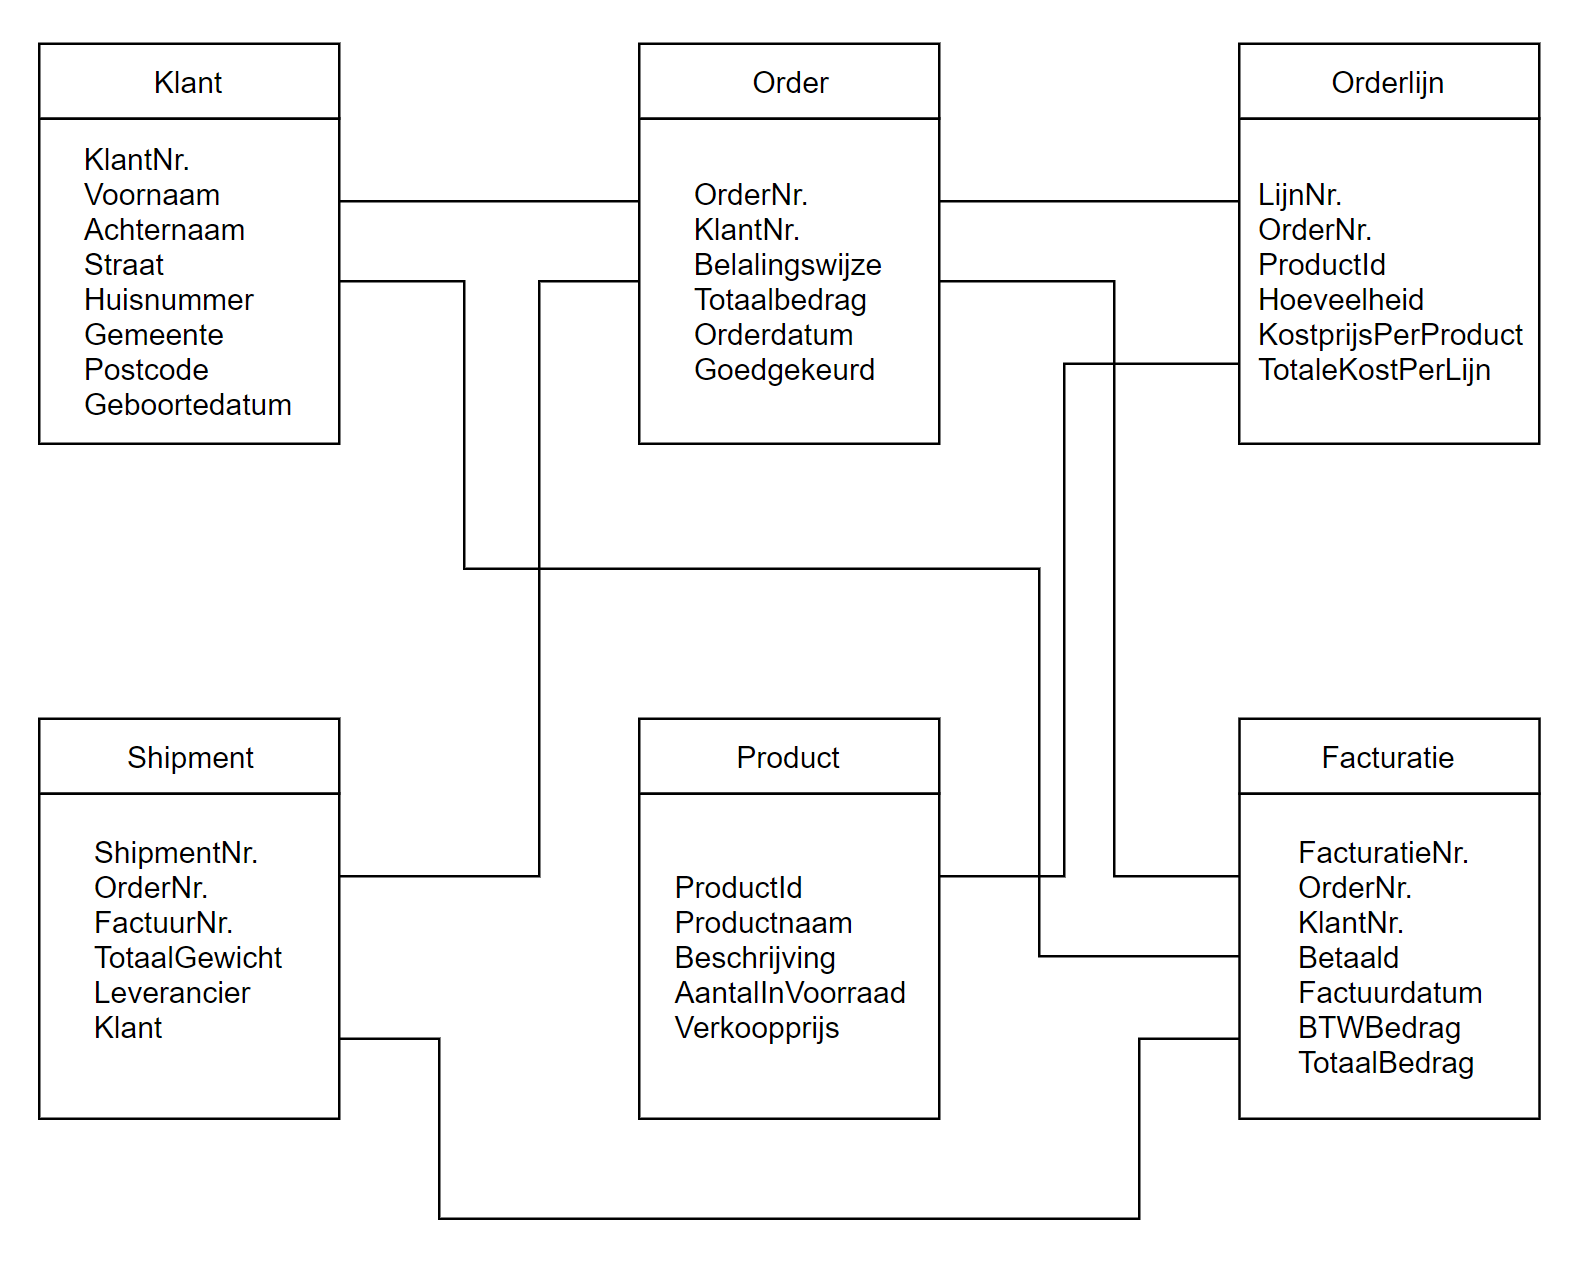
\includegraphics[height=.8\textheight]{img/databank.png}
		% Bron afbeelding: https://www.pexels.com/photo/hand-on-cup-of-coffee-984536/
		\label{img:databank}
	\end{figure}

\end{frame}

\begin{frame}
	\frametitle{De complete architectuur opbouwen}
	\begin{itemize}
		\item De architectuur
		\item De volgende stappen.
	\end{itemize}

\end{frame}

\begin{frame}
	\begin{figure}
		\caption{De architectuur}
		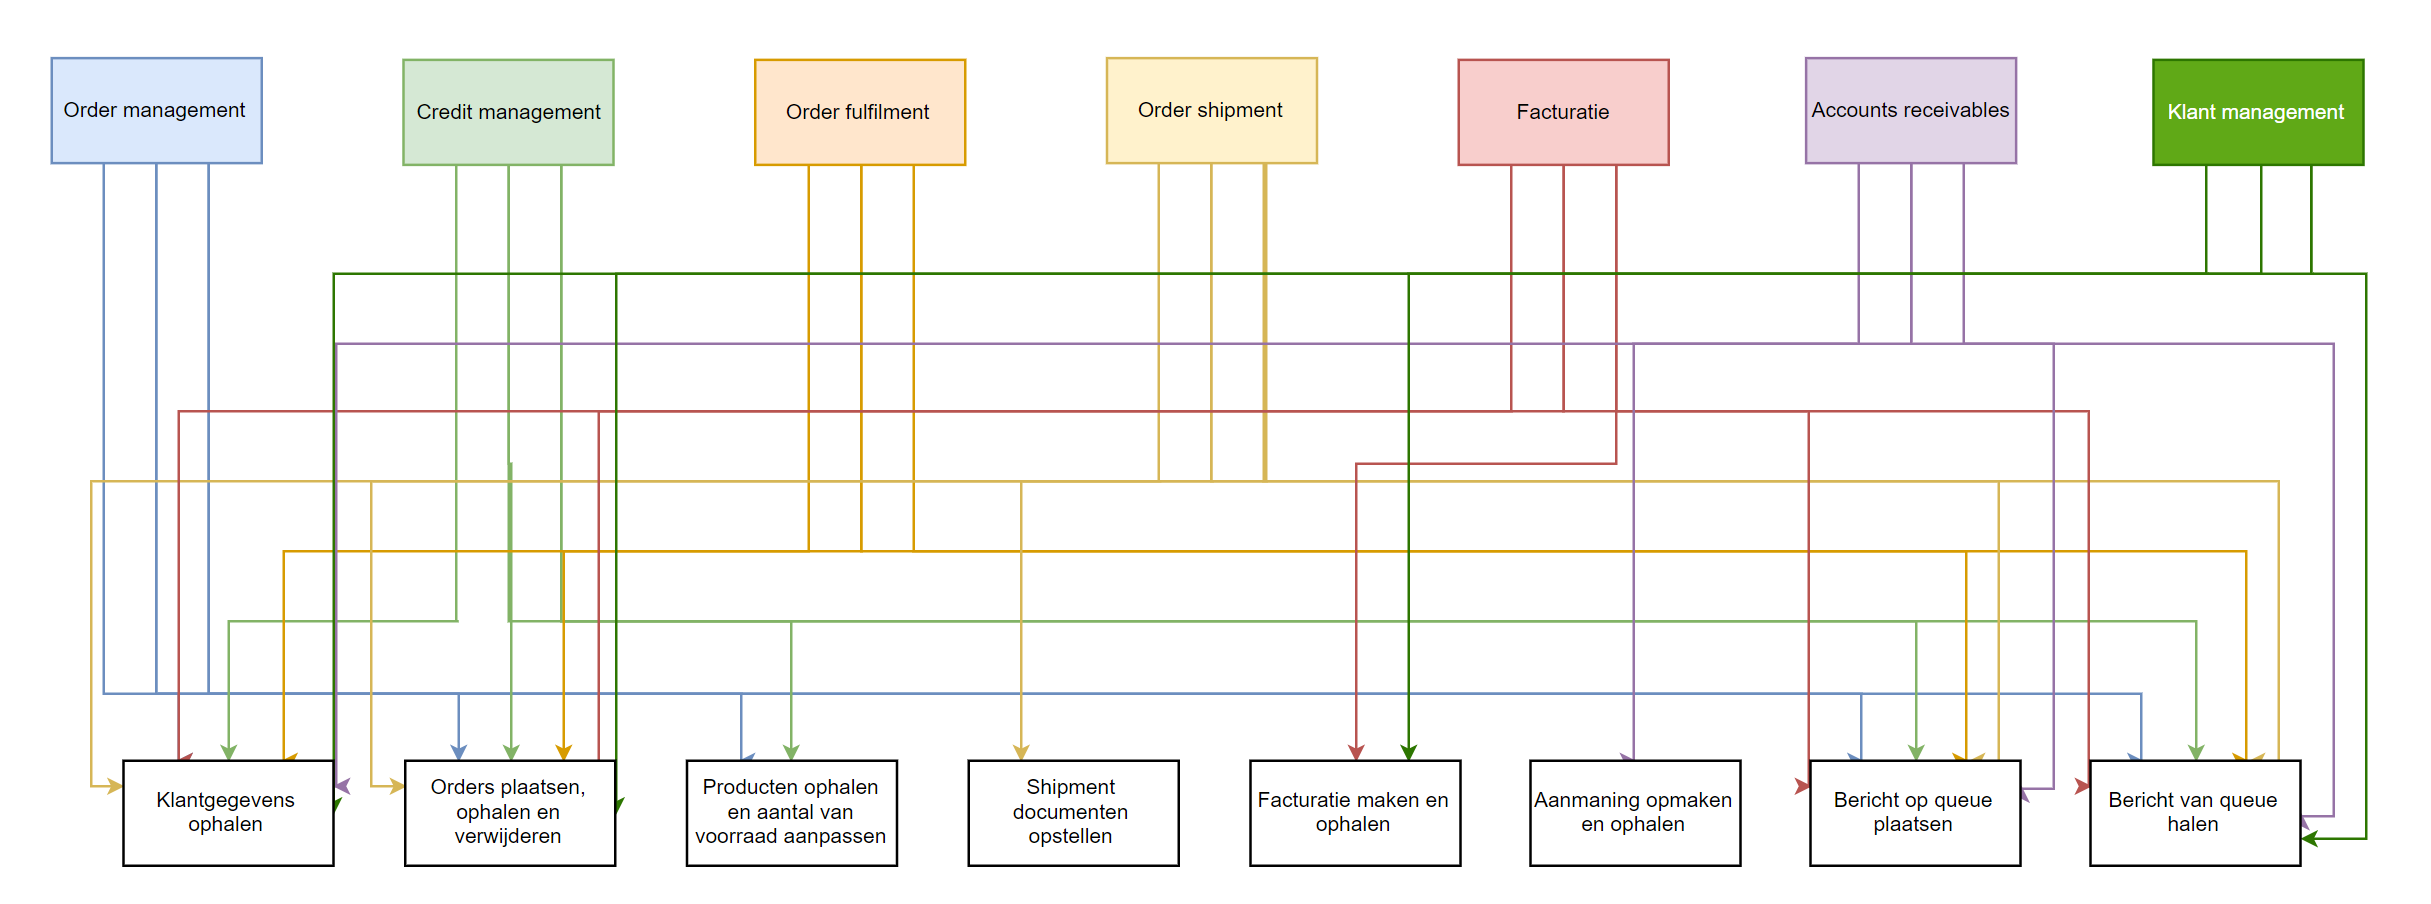
\includegraphics[height=.8\textheight]{img/schema_microservices.png}
		% Bron afbeelding: https://www.pexels.com/photo/hand-on-cup-of-coffee-984536/
		\label{img:microservices}
	\end{figure}
\end{frame}

\begin{frame}
	\begin{figure}
		\caption{Order management}
		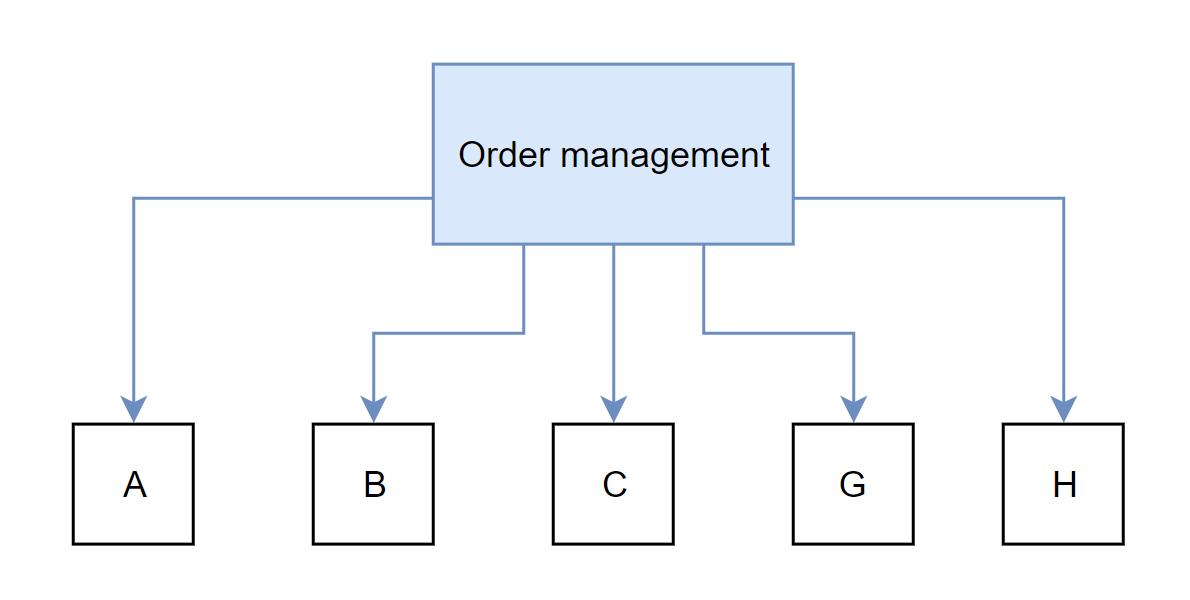
\includegraphics[height=.8\textheight]{img/ordermanagement.png}
		% Bron afbeelding: https://www.pexels.com/photo/hand-on-cup-of-coffee-984536/
		\label{img:order_management}
	\end{figure}
\end{frame}

\begin{frame}
\begin{figure}
	\caption{Credit management}
	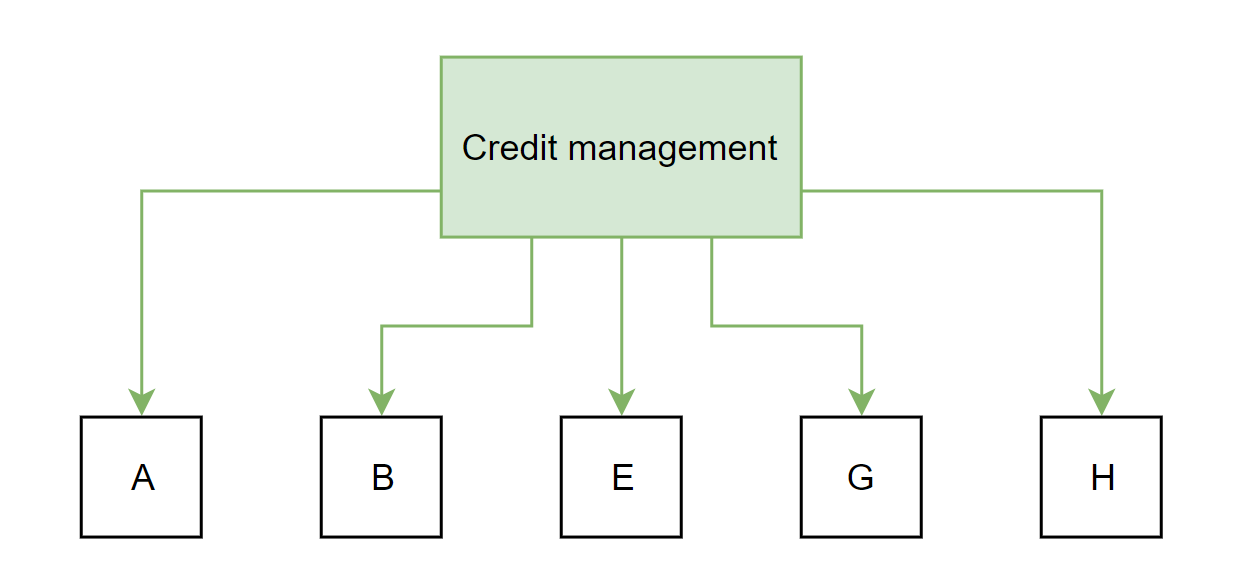
\includegraphics[height=.8\textheight]{img/creditmanagement.png}
	% Bron afbeelding: https://www.pexels.com/photo/hand-on-cup-of-coffee-984536/
	\label{img:credit_management}
\end{figure}
\end{frame}

\begin{frame}
\begin{figure}
	\caption{Order fullfilment}
	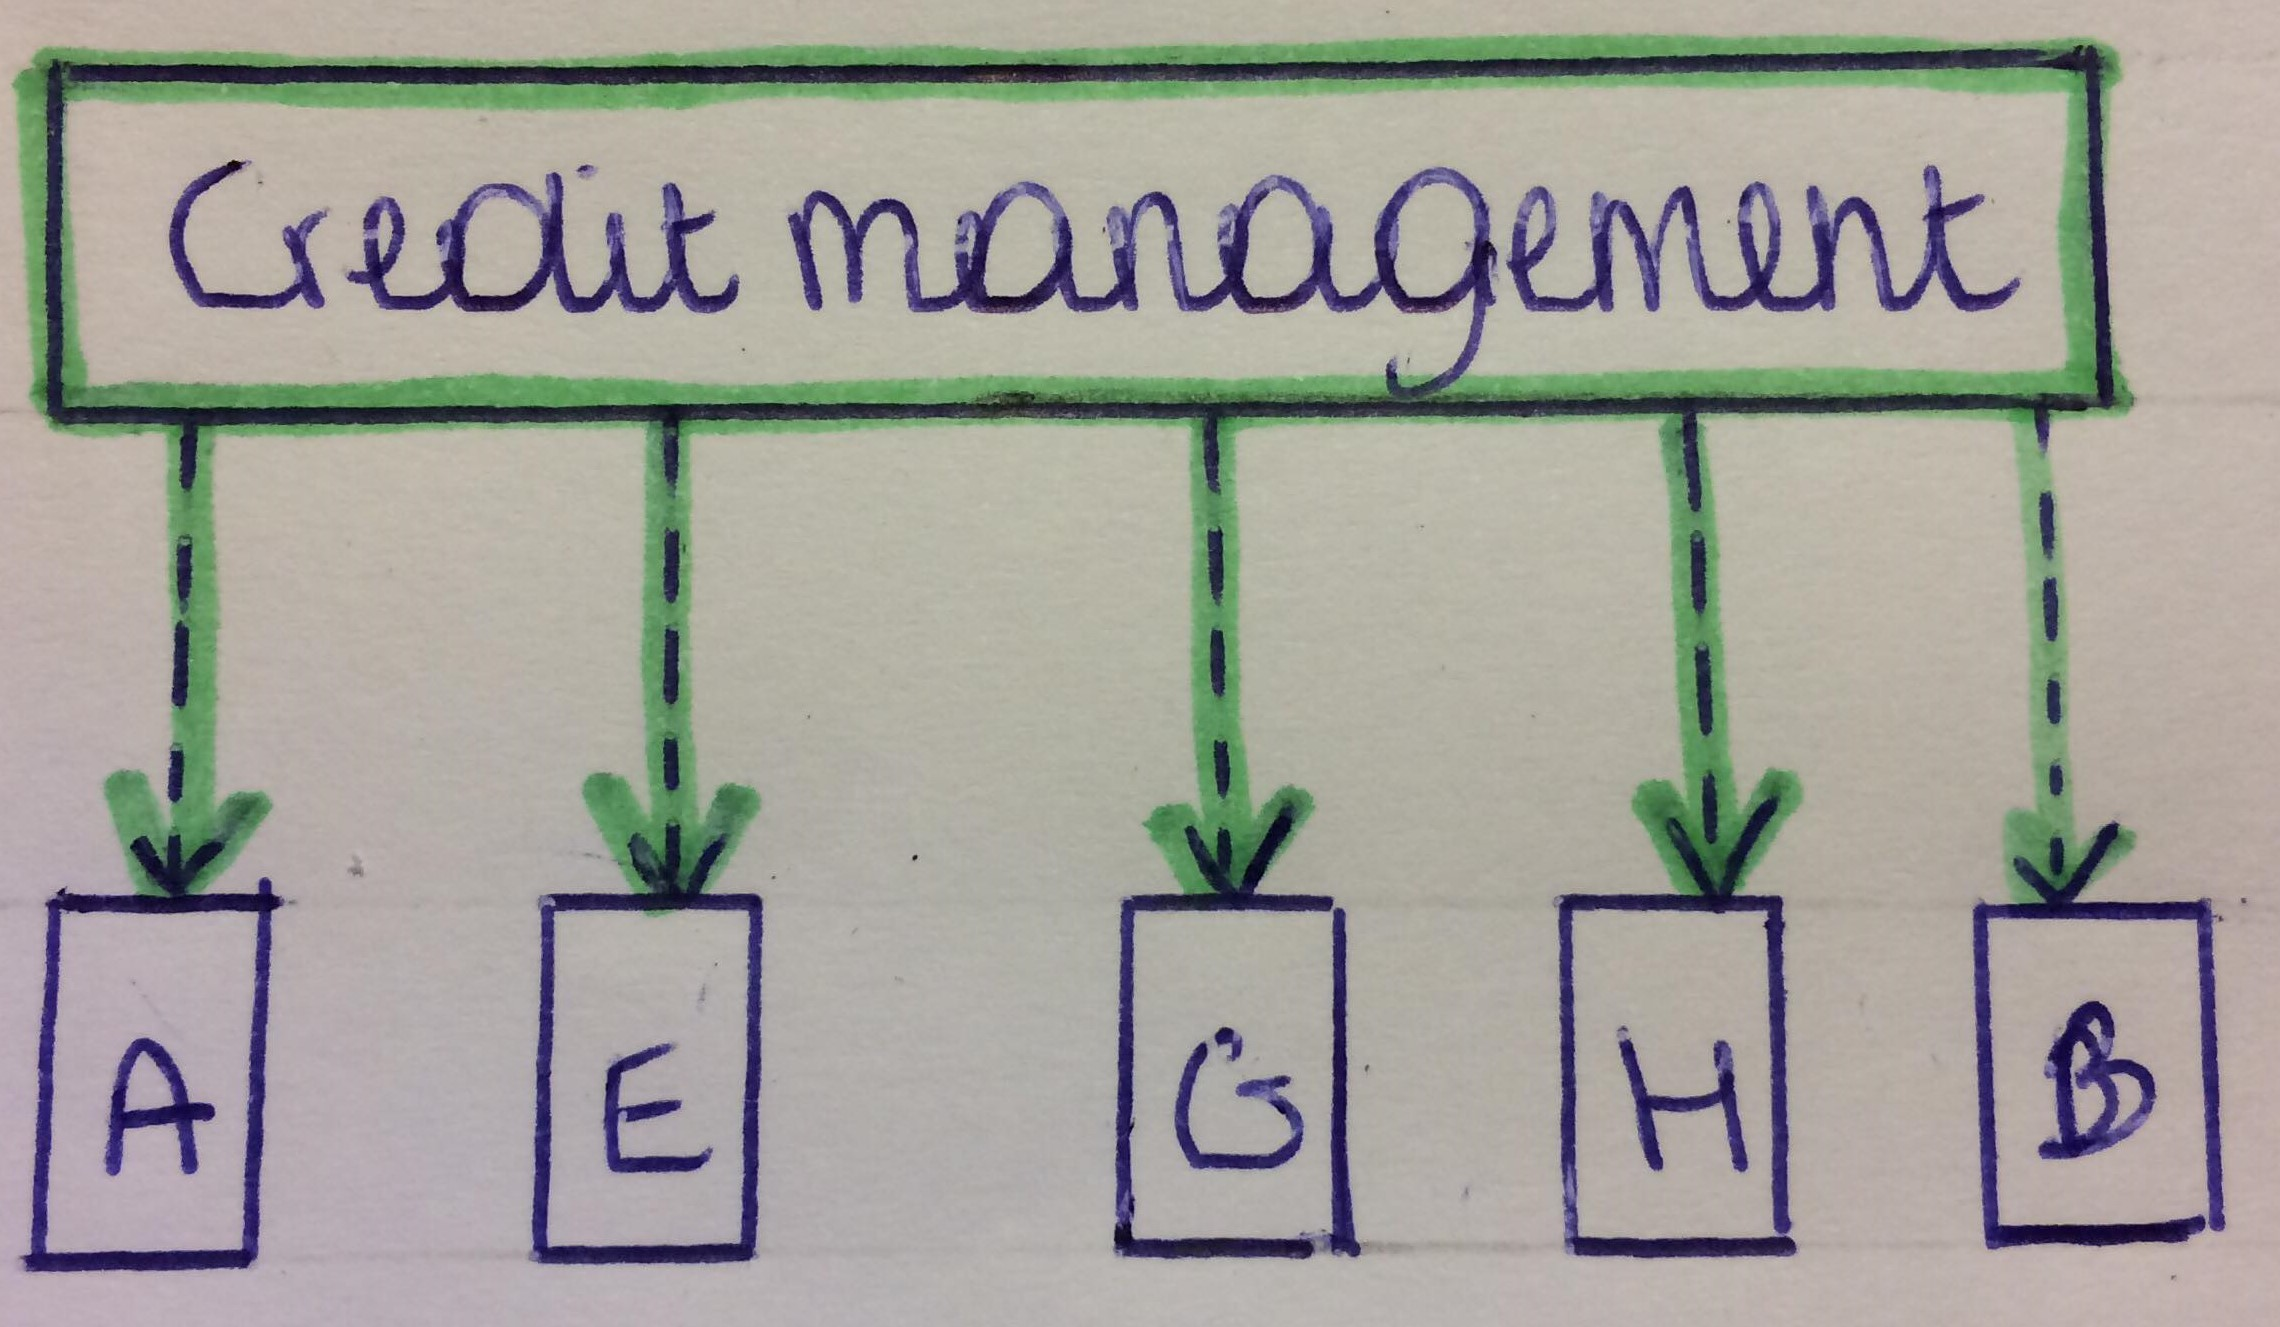
\includegraphics[height=.8\textheight]{img/orderfullfilment.png}
	% Bron afbeelding: https://www.pexels.com/photo/hand-on-cup-of-coffee-984536/
	\label{img:order_fullfilment}
\end{figure}
\end{frame}

\begin{frame}
\begin{figure}
	\caption{Order shipment}
	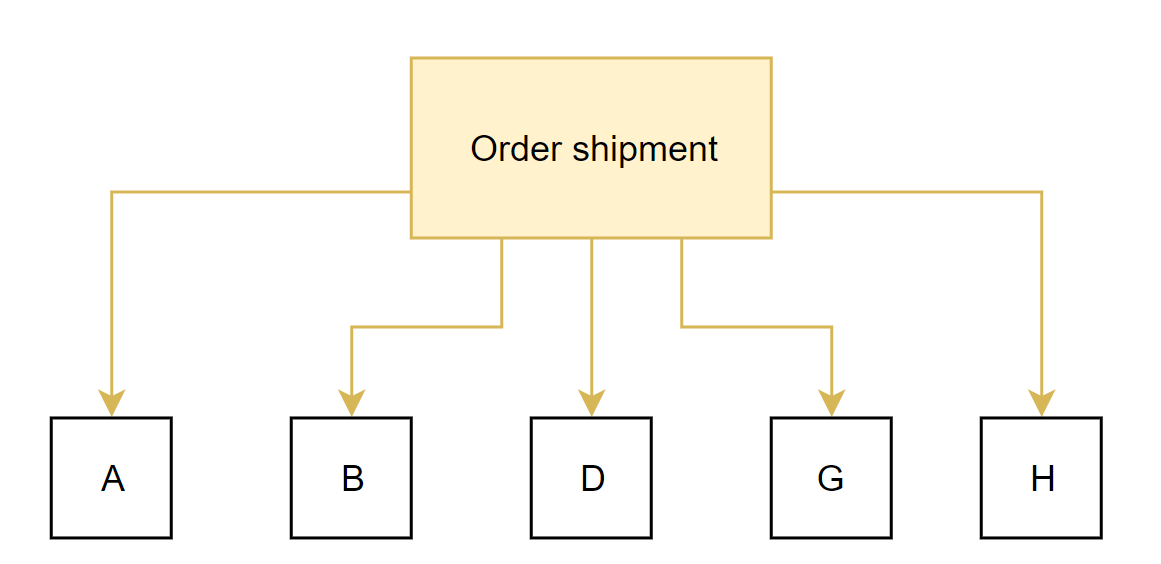
\includegraphics[height=.8\textheight]{img/ordershipment.png}
	% Bron afbeelding: https://www.pexels.com/photo/hand-on-cup-of-coffee-984536/
	\label{img:order_shipment}
\end{figure}
\end{frame}

\begin{frame}
\begin{figure}
	\caption{Facturatie}
	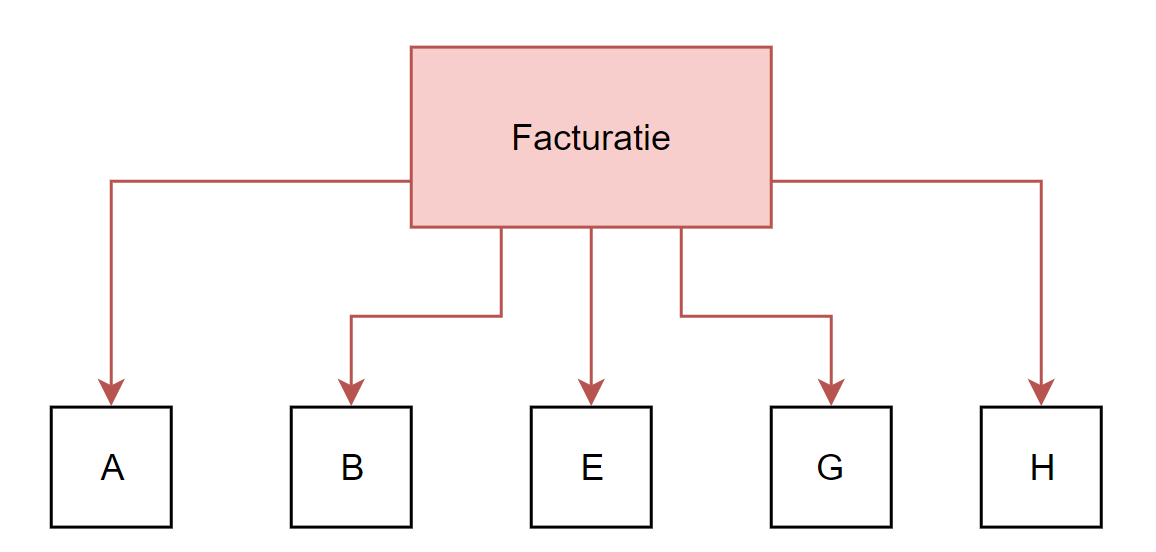
\includegraphics[height=.8\textheight]{img/facturatie.png}
	% Bron afbeelding: https://www.pexels.com/photo/hand-on-cup-of-coffee-984536/
	\label{img:facturatie}
\end{figure}
\end{frame}

\begin{frame}
\begin{figure}
	\caption{Accounts receivables}
	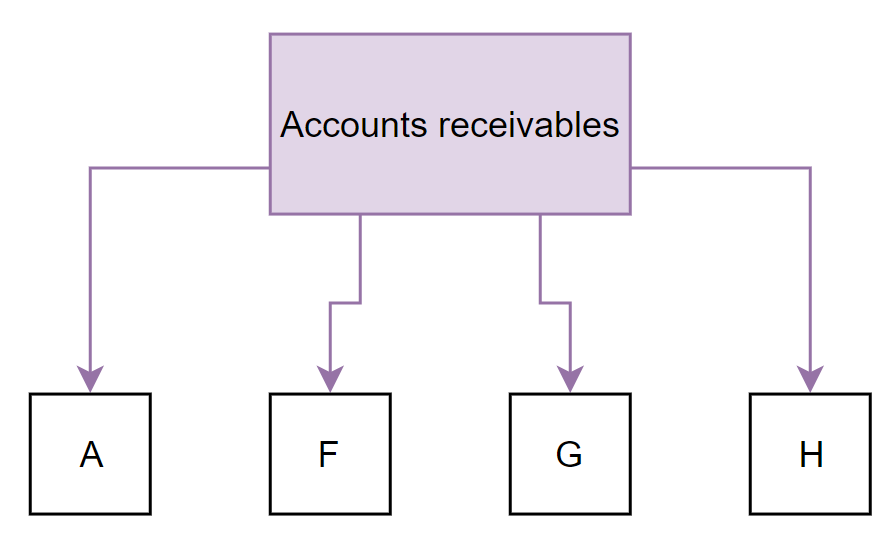
\includegraphics[height=.8\textheight]{img/accountreceivables.png}
	% Bron afbeelding: https://www.pexels.com/photo/hand-on-cup-of-coffee-984536/
	\label{img:accounts_receivables}
\end{figure}
\end{frame}

\begin{frame}
\begin{figure}
	\caption{Klant management}
	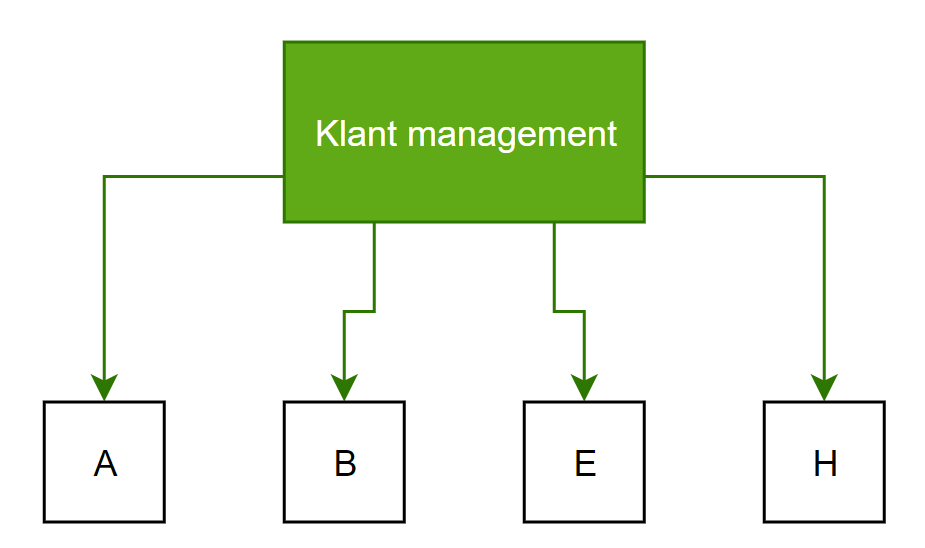
\includegraphics[height=.8\textheight]{img/klantmanagement.png}
	% Bron afbeelding: https://www.pexels.com/photo/hand-on-cup-of-coffee-984536/
	\label{img:klant_management}
\end{figure}
\end{frame}

\begin{frame}
	\frametitle{De volgende stappen}
	\begin{itemize}
		\item Logging toevoegen aan de architectuur
		\item Authenticatie en authorisatie
		\item Toevoegen van API gateway
	\end{itemize}
\end{frame}

\begin{frame}
	\frametitle{Toevoegen van API gateway}
	\begin{figure}
		\caption{Toevoegen API gateway}
		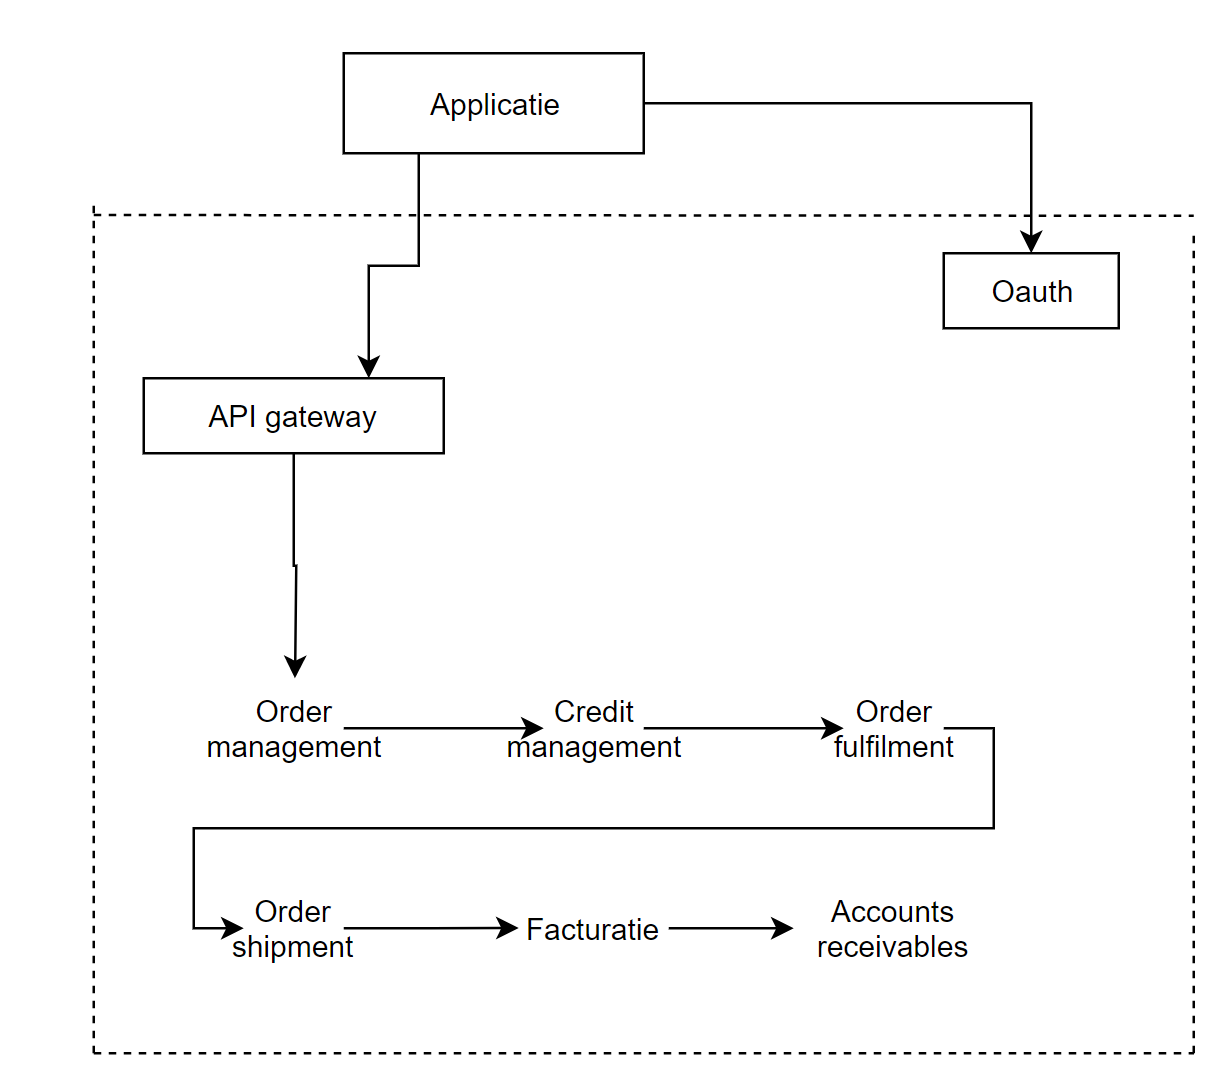
\includegraphics[height=.8\textheight]{img/apiSchema.png}
		% Bron afbeelding: https://www.pexels.com/photo/hand-on-cup-of-coffee-984536/
		\label{img:api_schema}
	\end{figure}
\end{frame}

%---------- CONCLUSIE ------------------------------------------------------------

\section{Conclusie}

\begin{frame}
\frametitle{Conclusie}
	\begin{itemize}
		\item Microservices is een brede term.
		\item Microservices kan voorkomen in verschillende contexten.
		\item De microservice architectuur is niet altijd nodig.
		\item Microservices kunnen een order-to-cash proces automatiseren.
		\item Dankzij microservices kan elk onderdeel apart functioneren.
	\end{itemize}

\end{frame}

\begin{frame}
	\frametitle{Bedankt voor het luisteren. Zijn er nog vragen?}
\end{frame}
\end{document}
